\section{Evaluation}
\FloatBarrier%

\subsection{Regularisation}
Since regularisation is very important to prevent overfitting, the common
methods of regularisation are tested first to obtain a good baseline value for the
rest of the experiments. These methods are:
\begin{itemize}
  \item Dropout, with values taken from the set
    $\left\{0.0, 0.1, 0.2, 0.3, 0.4, 0.5\right\}$.
  \item Weight decay, with values taken from the set
    \[
      \left\{0.0, \num{1e-5}, \num{1e-4}, \num{1e-3}, \num{1e-2}\right\}.
    \]
\end{itemize}
Further details on these methods are given in \cref{sec:method}.

\subsubsection{Dropout}
\Cref{fig:dropout_plots} shows the training loss over time, as well as the
resulting precision-recall curve on the training set. Other than the training
loss being higher with higher dropout values (which is to be expected), there
does not seem to be any difference in performance. This lack of effect is also
shown in \cref{fig:dropout_dists}. A dropout rate of 0.3 appears to score the
best, although none of the distributions are different in a statistically
significant way. The full data, with the mean and standard deviation of the F1
score and the area under the curve, are given in
\cref{tbl:dropout}.

\begin{figure}[htbp]
  \centering
  \begin{subfigure}[t]{0.49\textwidth}
    \centering
    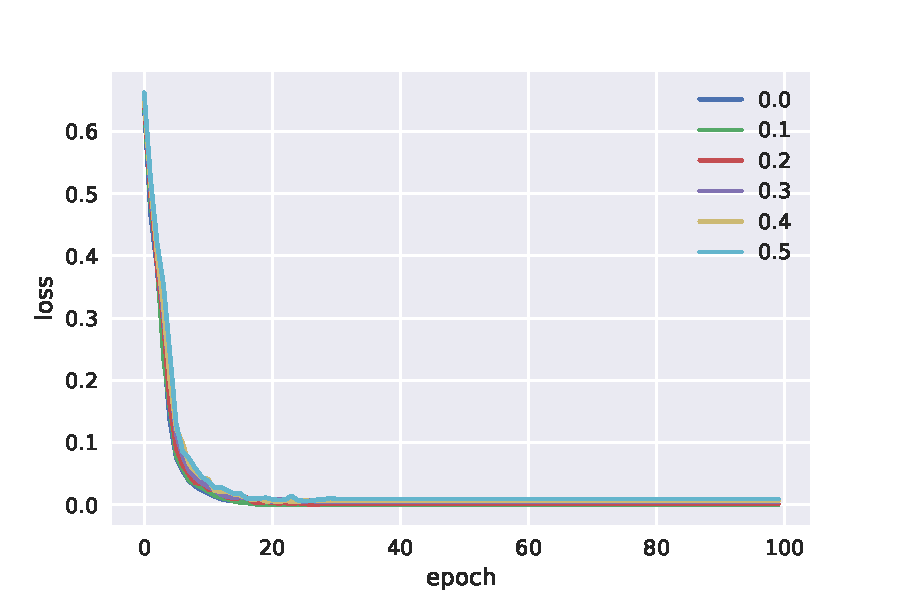
\includegraphics[width=\textwidth]{./figures/results/dropout/losses.pdf}
    \caption{The average loss at each epoch.\\}%
    \label{fig:dropout_loss}
  \end{subfigure}
  \begin{subfigure}[t]{0.49\textwidth}
    \centering
    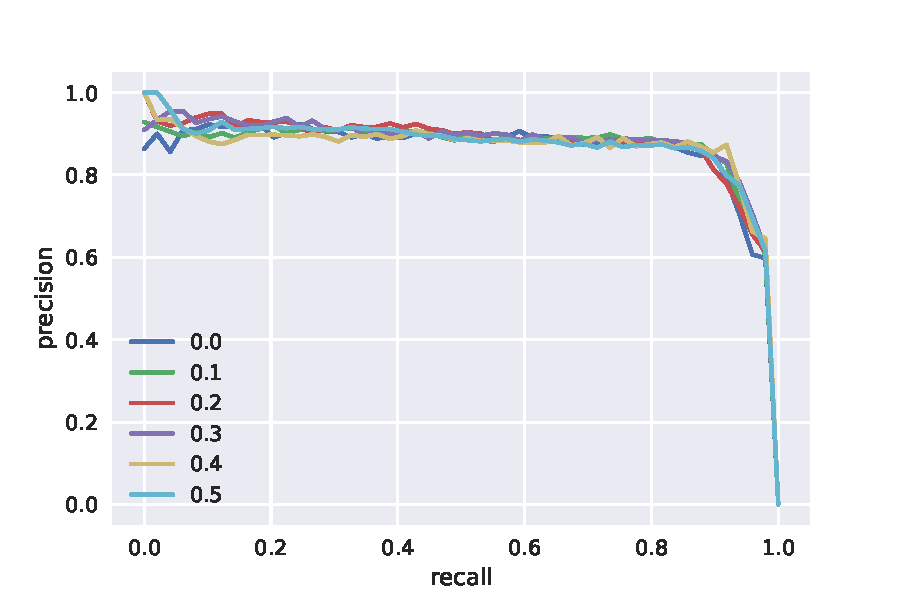
\includegraphics[width=\textwidth]{./figures/results/dropout/pr.pdf}
    \caption{The average precision-recall curves at various dropout values.}%
    \label{fig:dropout_pr}
  \end{subfigure}
  \caption{The loss over time (\subref{fig:dropout_loss}) and the
    precision-recall curve (\subref{fig:dropout_pr}). In both cases, the values are
    averaged over 10 trials.}%
    \label{fig:dropout_plots}
\end{figure}

\begin{figure}[htbp]
  \centering
  \begin{subfigure}[t]{0.49\textwidth}
    \centering
    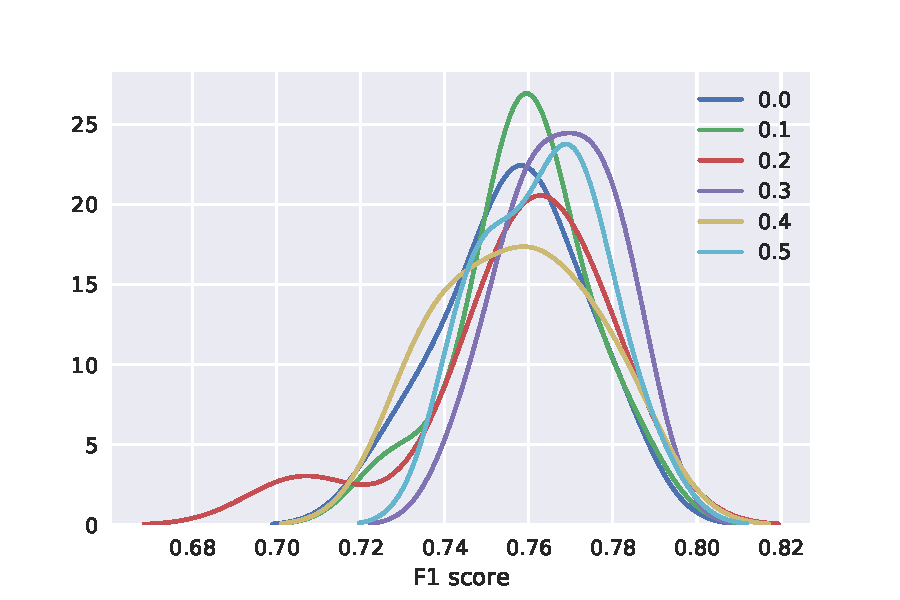
\includegraphics[width=\textwidth]{./figures/results/dropout/kde_f1.pdf}
    \caption{Kernel density estimation}%
    \label{fig:dropout_kde}
  \end{subfigure}
  \begin{subfigure}[t]{0.49\textwidth}
    \centering
    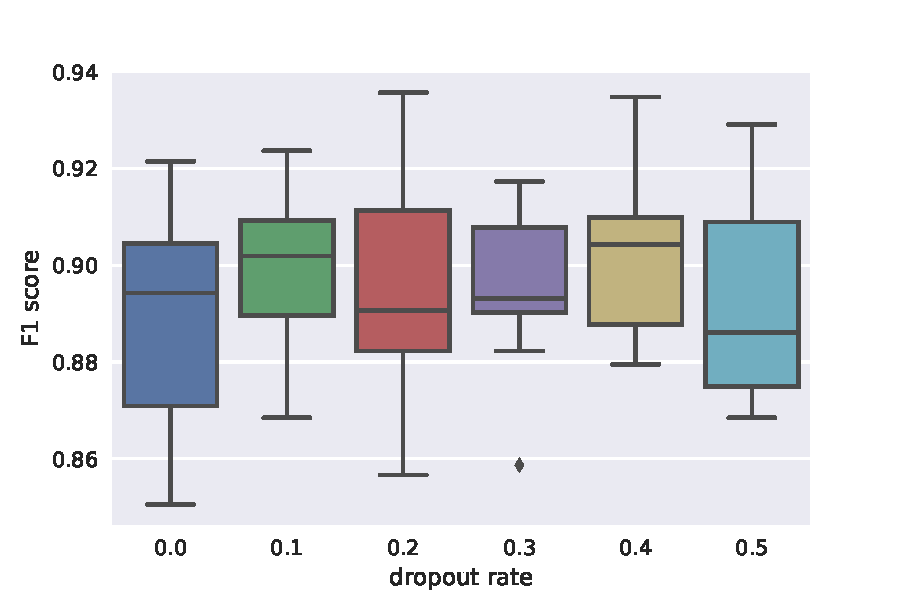
\includegraphics[width=\textwidth]{./figures/results/dropout/boxplot_f1.pdf}
    \caption{Boxplot}%
    \label{fig:dropout_box}
  \end{subfigure}
  \caption{A kernel density estimation and boxplot, based on the F1 score values
  over 10 repeated trials.}%
  \label{fig:dropout_dists}
\end{figure}

\begin{table}[htb]
  \centering
  \import{./figures/results/dropout/}{scores.tex}
  \caption{The F1 and AoC scores at various dropout values.}%
  \label{tbl:dropout}
\end{table}

\FloatBarrier%
\subsubsection{Weight decay}
Similarly to the dropout plots, \cref{fig:decay_plots} shows the training loss
over time and the precision-recall curve at various weight decay values. There
are again no significant differences, with a value of \num{1e-4} performing just
slightly better.

\begin{figure}[htbp]
  \centering
  \begin{subfigure}[t]{0.49\textwidth}
    \centering
    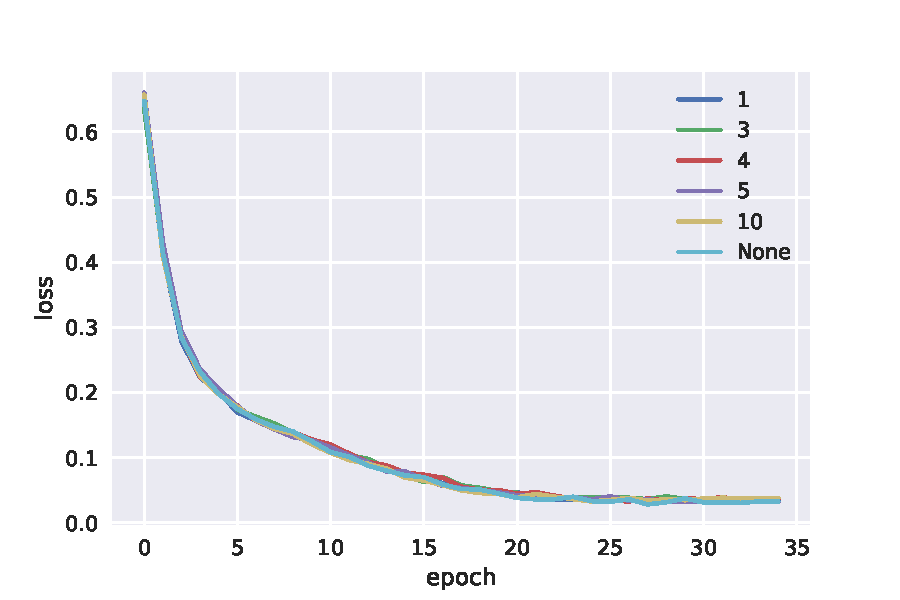
\includegraphics[width=\textwidth]{./figures/results/decay/losses.pdf}
    \caption{The average loss at each epoch.\\}%
    \label{fig:decay_loss}
  \end{subfigure}
  \begin{subfigure}[t]{0.49\textwidth}
    \centering
    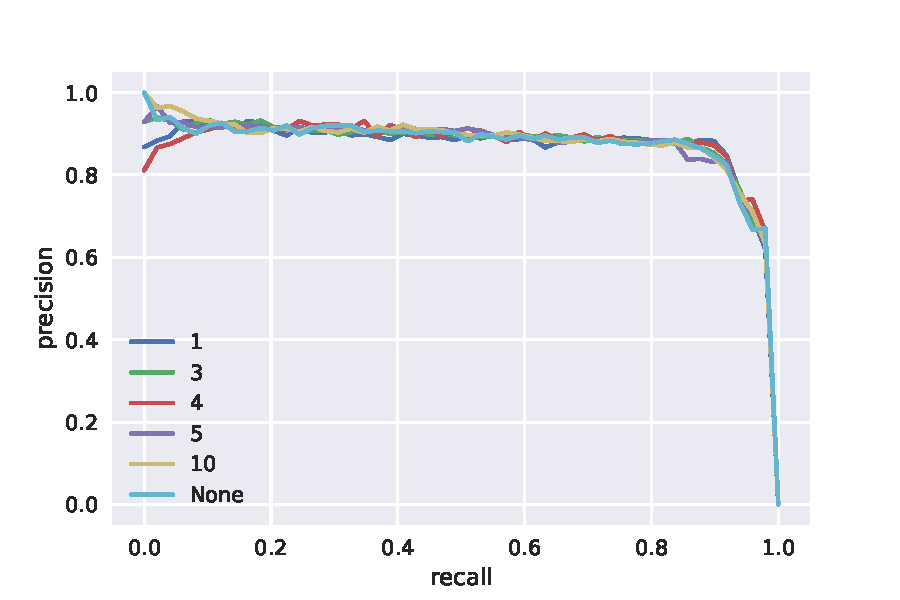
\includegraphics[width=\textwidth]{./figures/results/decay/pr.pdf}
    \caption{The average precision-recall curves at various decay values.}%
    \label{fig:decay_pr}
  \end{subfigure}
  \caption{The loss over time (\subref{fig:decay_loss}) and the
    precision-recall curve (\subref{fig:decay_pr}). In both cases, the values are
    averaged over 10 trials.}%
    \label{fig:decay_plots}
\end{figure}

\begin{figure}[htbp]
  \centering
  \begin{subfigure}[t]{0.49\textwidth}
    \centering
    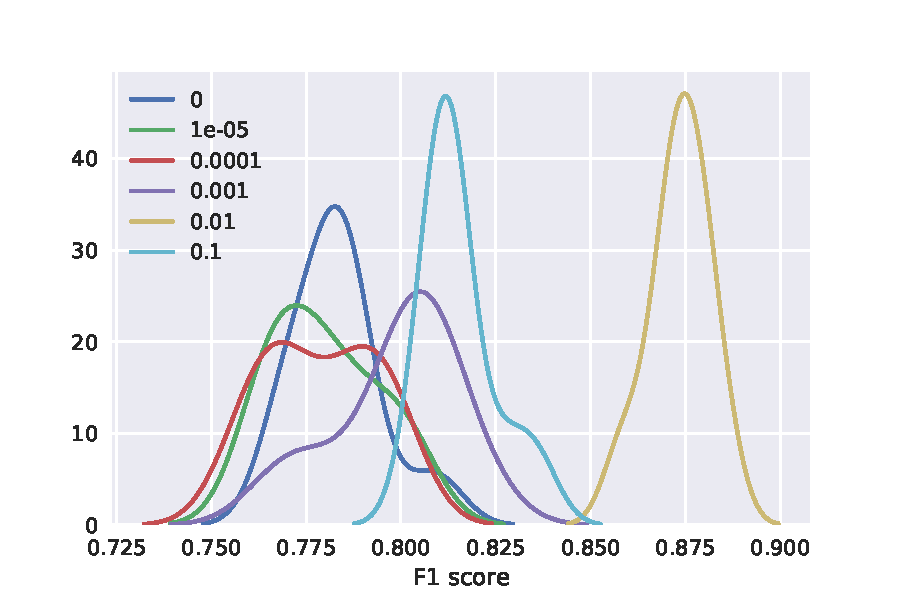
\includegraphics[width=\textwidth]{./figures/results/decay/kde_f1.pdf}
    \caption{Kernel density estimation}%
    \label{fig:decay_kde}
  \end{subfigure}
  \begin{subfigure}[t]{0.49\textwidth}
    \centering
    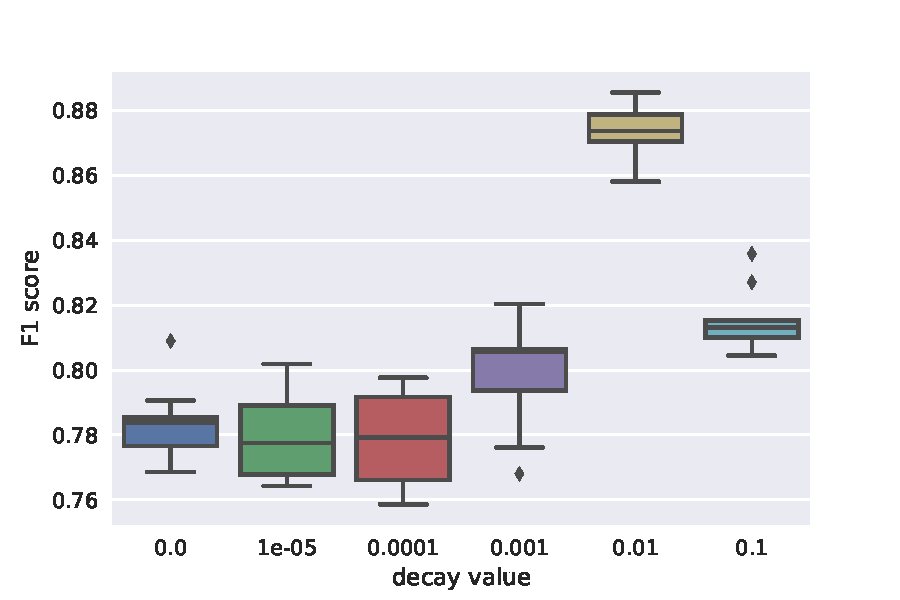
\includegraphics[width=\textwidth]{./figures/results/decay/boxplot_f1.pdf}
    \caption{Boxplot}%
    \label{fig:decay_box}
  \end{subfigure}
  \caption{A kernel density estimation and boxplot, based on the F1 score values
  over 10 repeated trials.}%
  \label{fig:decay_dists}
\end{figure}

\begin{table}[htb]
  \centering
  \import{./figures/results/decay/}{scores.tex}
  \caption{The F1 and AoC scores at various decay values.}%
  \label{tbl:decay}
\end{table}

\FloatBarrier%

\subsection{Models}
\begin{figure}[htbp]
  \centering
  \begin{subfigure}[t]{0.49\textwidth}
    \centering
    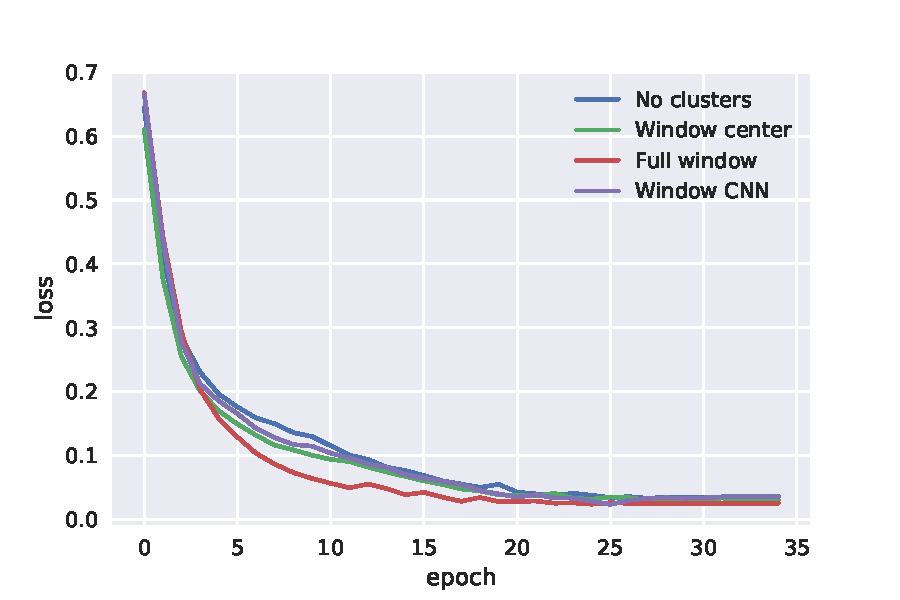
\includegraphics[width=\textwidth]{./figures/results/models/losses.pdf}
    \caption{The average loss at each epoch.\\}%
    \label{fig:model_loss}
  \end{subfigure}
  \begin{subfigure}[t]{0.49\textwidth}
    \centering
    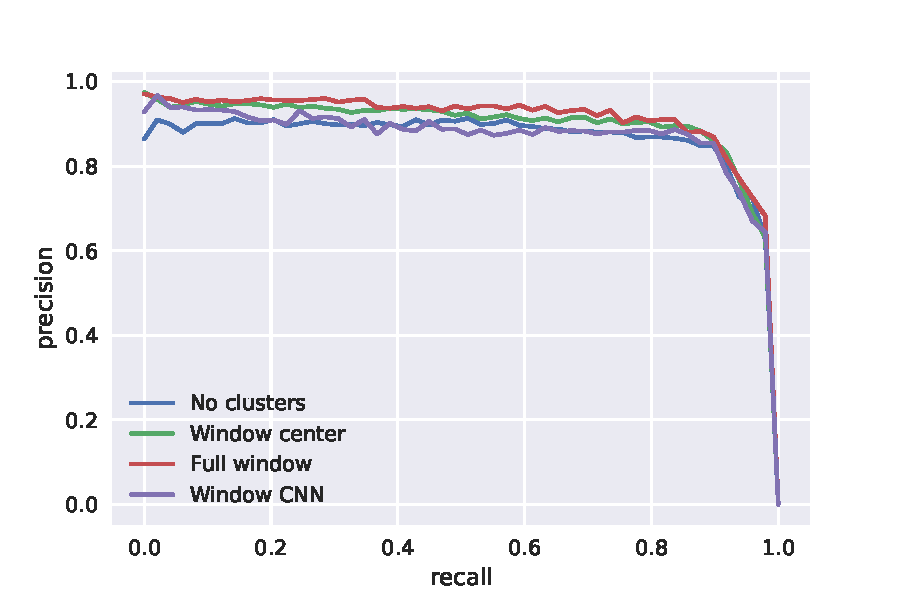
\includegraphics[width=\textwidth]{./figures/results/models/pr.pdf}
    \caption{The average precision-recall curves for the various models.}%
    \label{fig:model_pr}
  \end{subfigure}
  \caption{The loss over time (\subref{fig:model_loss}) and the
    precision-recall curve (\subref{fig:model_pr}). In both cases, the values are
    averaged over 10 trials.}%
    \label{fig:model_plots}
\end{figure}

Here the models described earlier (TODO: beschrijven en ernaar verwijzen) are
tested with the default parameters of the CNN\@. Based on the previous results,
the dropout rate was set to 0.3 and the decay to \num{1e-4}.
The plots in \Cref{fig:model_plots} show a subtle but observable difference; the
model using the full window jumps out of the pack in both cases, converging a
little bit faster and being on top for most of the precision-recall curve,
although the model with an additional CNN catches up at higher recalls.

\begin{figure}[htbp]
  \centering
  \begin{subfigure}[t]{0.49\textwidth}
    \centering
    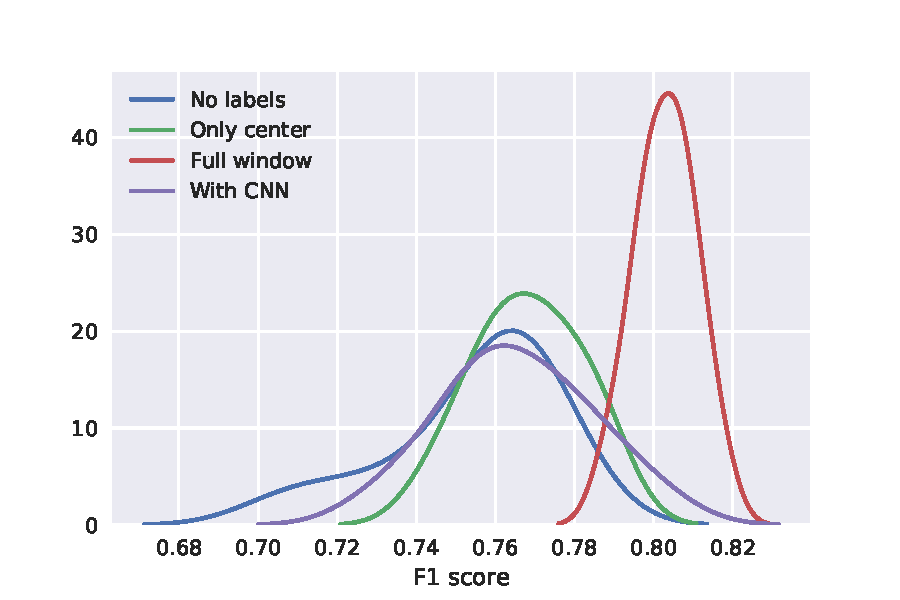
\includegraphics[width=\textwidth]{./figures/results/models/kde_f1.pdf}
    \caption{Kernel density estimation}%
    \label{fig:model_kde}
  \end{subfigure}
  \begin{subfigure}[t]{0.49\textwidth}
    \centering
    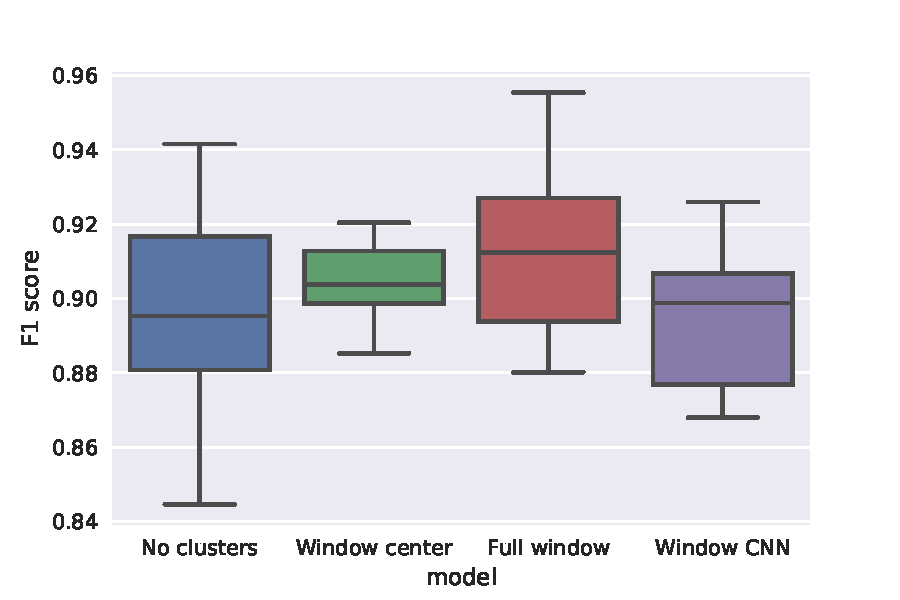
\includegraphics[width=\textwidth]{./figures/results/models/boxplot_f1.pdf}
    \caption{Boxplot}%
    \label{fig:model_box}
  \end{subfigure}
  \caption{A kernel density estimation and boxplot, based on the F1 score values
  over 10 repeated trials.}%
  \label{fig:model_dists}
\end{figure}

The boxplot in \cref{fig:model_box} paints a clear picture with three tiers of
performance: the model without cluster labels performs worst, adding only the
cluster of center of the window improves it a bit, while using the full window
performs best with and without a CNN applied to it.
\Cref{fig:model_dists} showns an interesting relation between the two top
performing models. Their score distributions are clearly bimodal with both peaks
occurring at roughly the same scores, indicating the possibly of getting caught
in a local optimum. The real win of the simpler model without the CNN appears to
be that it is far less likely to get stuck in that local optimum.

\begin{table}[htb]
  \centering
  \import{./figures/results/models/}{scores.tex}
  \caption{The F1 and AoC scores of the various models.}%
  \label{tbl:model}
\end{table}

Significance values for the F1 score are given in \cref{tbl:model_sign}, which
shows that every model is different from every other model using the common
cutoff of $p <= 0.05$. The least convincing is the difference between the two
best models (Full window and Window CNN), but given the still significant result
it is reasonable to state that the Full window model is the clearly winner given
its far more reliable ability to reach the global optimum.

\begin{table}[htb]
  \centering
  \import{./figures/results/models/}{f1_sign.tex}
  \caption{The probability for each pair of models that their F1 scores are
  generated by the same underlying distribution (i.e.\ the probability of the
  null hypothesis that the models perform the same being true).}%
  \label{tbl:model_sign}
\end{table}

\subsection{Number of clusters}
\Cref{fig:kmeans_box} shows the results of varying the number of clusters
created in the final k-means clustering step.
\begin{figure}[htbp]
  \centering
    \centering
    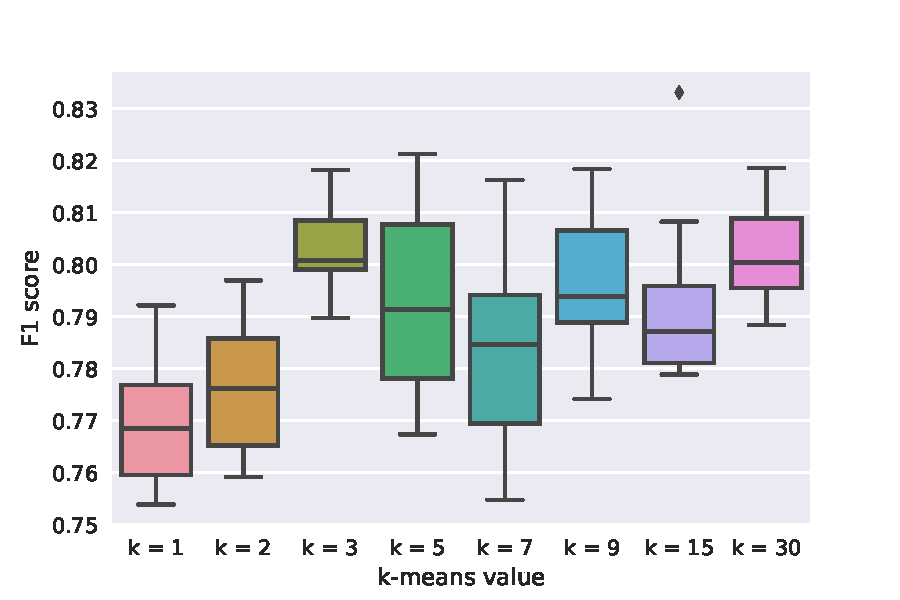
\includegraphics[width=\textwidth]{./figures/results/kmeans/boxplot_f1.pdf}
    \caption{A boxplot based on the F1 scores of 10 repeated trials for various
    amounts of clusters created by the k-means algorithm.}%
    \label{fig:kmeans_box}
\end{figure}

\FloatBarrier%

%%% Local Variables:
%%% mode: latex
%%% TeX-master: "report"
%%% End:
